%This section needs to be changed a lot
%Lets break it down into 'validation' and put that in the previous section
%
%I am adding another section which talks about the 'main' simulation

\section{Validation} %TODO: no longer a chapter

In this section, there will be two subsections.  One will discuss the simulation to validate our design and implementation.  
% TODO: reword - two stages in the simulation process -> not two sections in the report
The other will be used to test the performance using parametric studies.  
More detail will be explained in the following subsequent section \ref{sec:scenario1} and \ref{sec:scenario2}.

Some pa
We define our packet loss as the number of packets dropped due to the fact that the buffer size limit has been reached.


%When simulating each scenario, the following metrics will be measured:
%\begin{enumerate}
%	\item Time to update state in central repository (delay)
%	\item Variation in time to update state (delay jitter)
%	\item Number of state updates lost. Roughly corresponds to packet loss.
%	\item Memory utilization and packet dropping threshold within ferries.
%\end{enumerate}

%_________________________________________________________________
%________________________SCENARIO 1_______________________________
\subsection{Scenario 1: Validation}
\label{sec:scenario1}

In this scenario, we are trying to test our design implementation, we need to address what to look for.  
% Dont use 'we', dont refer to section -> stage
% Not what to look for -> validate that the node models work 
We need to validate that the updates from source nodes are delivered successfully when in range and to see if the packets are handled properly as designed.  

\subsubsection{Topology}

The speed of the ferries is random and the direction is random, where the speed is within 36kph to 72kph in a uniform distribution.  
% No: constant speed of 60 kph

In Figure \ref{fig:scenario1}we test to see if the gateway receives the update packets sent by the source nodes.  
There are two gateway nodes, two ferry nodes, and seven source nodes.  
The directions of each ferry are indicated by red arrows.
The paths of the ferry movement is outlined in white color.

%picture of the rectangular path
\begin{figure}[h]
    \centering
    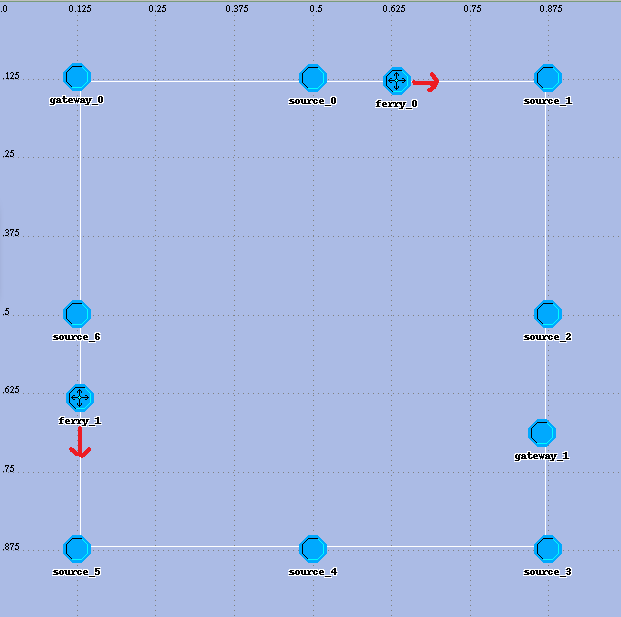
\includegraphics[width=.7\textwidth]{images/scenario1-top2}
    \caption{Scenario1 Topology2}
    \label{fig:scenario1}
\end{figure}

The simulation run time is 6 minutes.  

\subsubsection{Simulation 1 Results}
%The results you show here are for a different simulation

After setting up OPNET to capture the desired statistics, we simulate our design and see if it is successful in delivering packets from the source nodes to the gateway node.

%result1-a   ferry receives update packets
\begin{figure}[h]
    \centering
    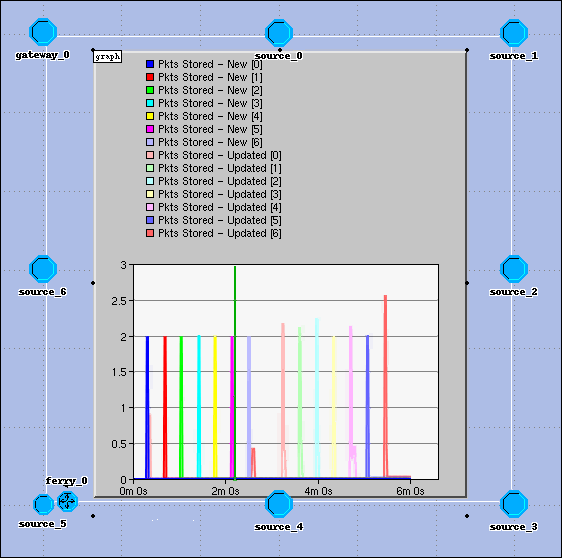
\includegraphics[width=.5\textwidth]{images/scenario1-result-received}
    \caption{Scenario1 packets received as the ferry moves along the rectangular path}
    \label{fig:result1-a}
\end{figure}

In Figure \ref{fig:result1-a}, we have the ferry moving in clockwise again in the defined path, highlighted in white.  
From Figure \ref{fig:result1-b}, there are two spikes in the graph which corresponds to the task of dumping the packets to the gateway node.  
The ferry node goes around two times for this simulation and that is why we see we two spikes.  
Each source node sends three update packets to the ferry node as it passes.  
Since there are seven source nodes, this accounts for the 20 packets received by the gateway node, which can be seen in Figure \ref{fig:result1-b}.


%result1-b   ferry delivers update packets to gateway
\begin{figure}[h]
    \centering
    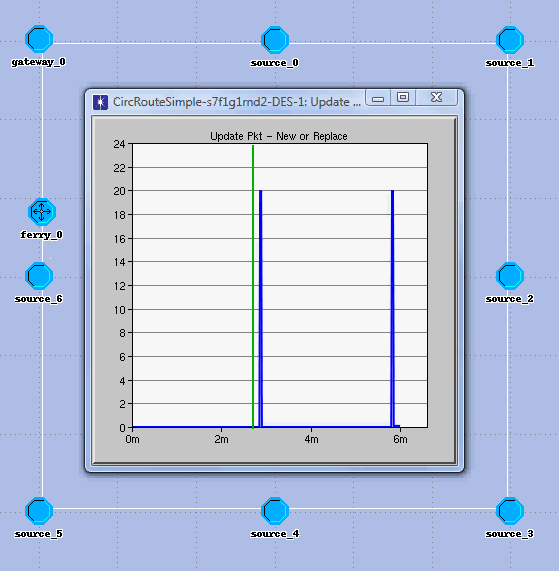
\includegraphics[width=.5\textwidth]{images/scenario1-result-gateway}
    \caption{Gateway receives the packet as the ferry node passes by its range of transmission}
    \label{fig:result1-b}
\end{figure}




%_________________________________________________________________
%________________________SCENARIO 2_______________________________
\subsection{Scenario 2 : Performance Evaluations}
\label{sec:scenario2}

%Basic introduction - a realistic situation
%	- random ferry movements

In this section, we examine the performance evaluations of message ferrying design to focus two parameters.  
One of them is to determine a so-called packet loss where we measure the memory utilization versus the packet dropping threshold within ferries.
% Not utilization - we are imposing a limit
Because of the nature of our algorithm, there may be dropped packets when the update number is older.
% Dont use 'our'
This loss measures the case where the buffer is full, and the oldest packets are dropped to accommodate for adding the new packet.  
The other is to find the delay, which is measured by the time to update the central repository.

\subsubsection{Scenario Considerations}

The following factors have been considered when designing scenarios:
\begin{itemize}
\item Number of sources to ferries to gateways (various ratios)
\item Speed and trajectories of ferries (random vs set path)
\item Rate of source node state changes
%\item Buffer size of ferries and size of property values (affects packet sizes)
%\item Distances and distributions of ferries and gateways
\end{itemize}

\subsubsection{Scenario 2: Topology}

In Figure \ref{fig:scenario2}, our scenario for the packet The size of this topology is 1km x 1km.  
That is the distance between source node 0 and 4 is 1km, while the distance between source node 6 and 2 is also 1km.  
The speed of the ferries is random and the direction is random, where the speed is within 36kph to 72kph in a uniform distribution.  

%overview of the scenario2 (random movement)
\begin{figure}[h]
    \centering
    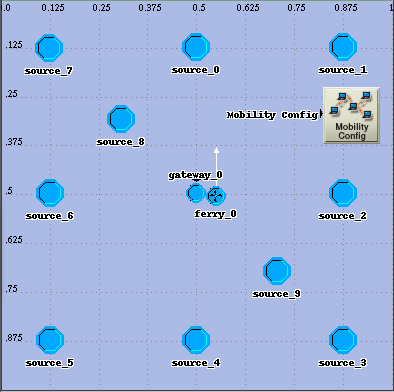
\includegraphics[width=.5\textwidth]{images/scenario2-top}
    \caption{Topology of Scenario 2}
    \label{fig:scenario2}
\end{figure}


\subsection{Results - Not here}

In the following graph, we can see that the buffer size used is proportional to the rate of successful packets delivered to ferries.

%graph of results for buffer size vs. packet loss [uncomment this when ready]
%\begin{figure}[h]
%    \centering
%    \includegraphics[width=.5\textwidth]{images/result1}
%    \caption{Buffer size versus packet drop rate }
%    \label{fig:result2}
%\end{figure}

This result was what we expected.  
The increase of the buffer size used resulted in fewer packet dropouts.



%gateway scenario
The increase of the number of gateways reduced the delay of updating to central repository.  
This result was expected because we knew that by properly placing another gateway in the area will grant better coverage.  
